% *******************************************************************************
% * Copyright (c) 2007-2008 by Elexis
% * All rights reserved. This document and the accompanying materials
% * are made available under the terms of the Eclipse Public License v1.0
% * which accompanies this distribution, and is available at
% * http://www.eclipse.org/legal/epl-v10.html
% *
% * Contributors:
% *    G. Weirich - initial implementation
% *
% *  $Id: konsviews.tex 3329 2007-11-07 17:44:06Z rgw_ch $
% *******************************************************************************

% !Mode:: "TeX:UTF-8" (encoding info for WinEdt)
\section{Elexis-Befunde}
\label{befunde}
\index{Befunde}\index{Quick-Reihen}
Einbindung textorientierter datierter Befundserien (z.B. Gewicht, BZ, Quick, Röntgenbefunde etc.). \subsection{Konfiguration}

\begin{figure}[htbp]
   \begin{minipage}{0.35\textwidth}
       \centering
       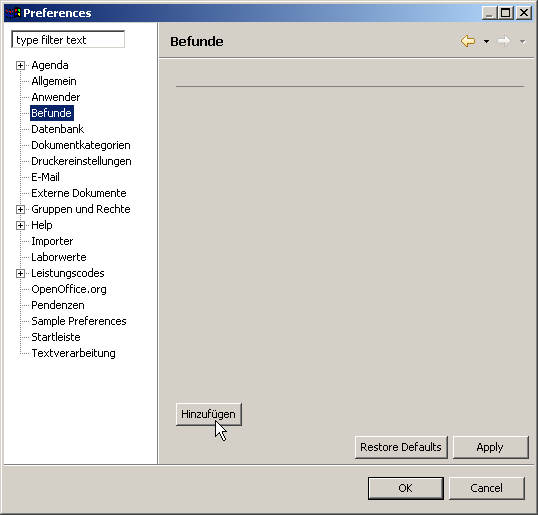
\includegraphics[width=0.9\textwidth]{images/befunde1}
       \caption{Befund}
       \label{fig:befundesettings}
     \end{minipage}\hfill
     \begin{minipage}{0.65\textwidth}
     Wenn das Plugin installiert ist, finden Sie im Menu Datei-Einstellungen eine Rubrik \textit{Befunde}. Diese wird anfangs leer sein (Abb. \ref{fig:befundesettings}).\\

     Um einen neuen Befundparameter hinzuzufügen, klicken Sie auf  \textit{Hinzufügen}. Sie werden nach dem Namen dieses Parameters gefragt, wir wählen  Röntgen. Danach erscheint eine Karteikarte mit diesem Parameter, die wir jetzt noch mit den einzutragenden Datenspalten versehen müssen.

    \end{minipage}
\end{figure}
\begin{figure}[htbp]
   \begin{minipage}{0.35\textwidth}
       \centering
        % befunde2.png: 538x515 pixel, 96dpi, 14.23x13.62 cm, bb=0 0 403 386
       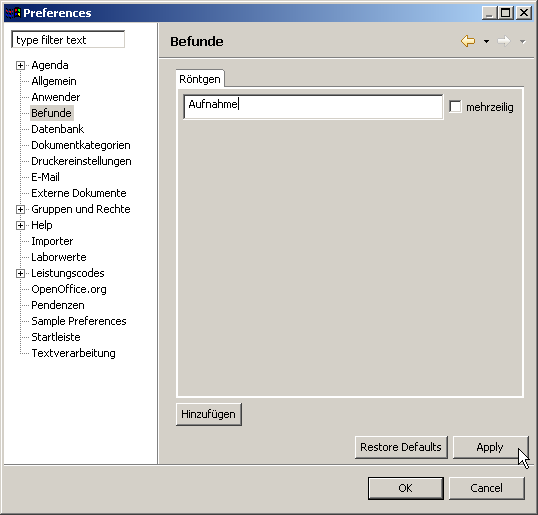
\includegraphics[width=0.9\textwidth]{images/befunde2}
       \caption{Parameter 2}
       \label{fig:befundesettings}
     \end{minipage}\hfill
     \begin{minipage}{0.65\textwidth}
        Klicken Sie nach jeder Zeile auf  \textit{Apply}  bzw.  \textit{Anwenden}:
        Wenn ein Feld mehrzeilig sein soll, klicken Sie die entsprechende Checkbox an. Eine Variante mit mehr als zwei Spalten sehen Sie in Abb. \ref{fig:befunde4}.:

    \end{minipage}
\end{figure}
\begin{figure}[htbp]
   \begin{minipage}{0.35\textwidth}
       \centering
    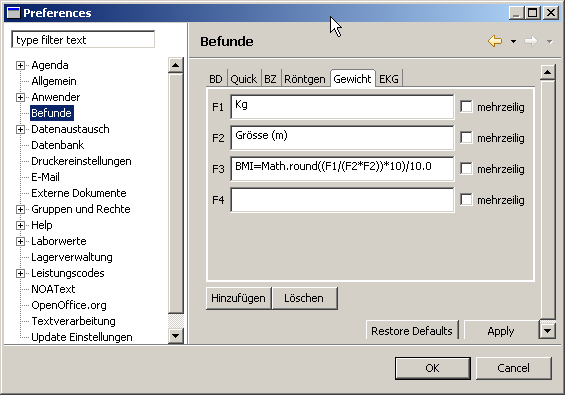
\includegraphics[width=0.9\textwidth]{images/befunde7.png}
    % befunde7.png: 580x520 pixel, 96dpi, 15.34x13.76 cm, bb=0 0 435 390
    \caption{Mehrspaltig}\label{fig:befunde4}
       \label{fig:befunde4}
     \end{minipage}\hfill
     \begin{minipage}{0.65\textwidth}
Werte können auch errechnet statt direkt eingegeben werden. Geben Sie hierzu einfach einen Ausdruck der Form \textit{Resultat=Formel} ein, wobei Sie sich mit Fx auf andere Felder derselben Seite beziehen können. Im Beispiel links errechnen wir den BMI aus den eingegebenen Werten für Grösse und Gewicht. Das Resultat wird allerdings standardmässig auf 9 Stellen genau ausgegeben, deswegen runden wir es hier auf eine Stelle.
    \end{minipage}
\end{figure}

\clearpage

\subsection{Anwendung}
Öffnen Sie die  Befunde-View.
\begin{flushleft}
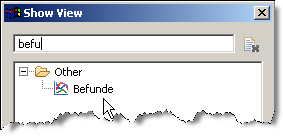
\includegraphics[width=3in]{images/befunde4.png}
% befunde4.png: 276x394 pixel, 96dpi, 7.30x10.42 cm, bb=0 0 207 295
\end{flushleft}

Sie sehen dann die konfigurierten Messparameter:
\begin{flushleft}
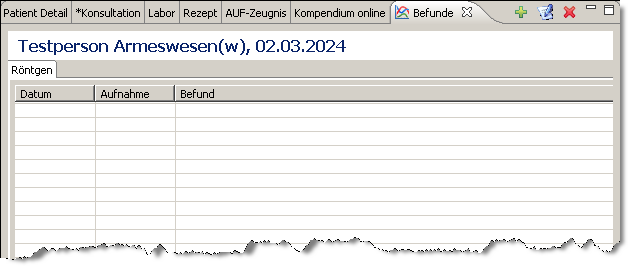
\includegraphics[width=4in]{images/befunde5.png}
% befunde5.png: 621x636 pixel, 96dpi, 16.43x16.83 cm, bb=0 0 466 477
\end{flushleft}
Um eine neue Messung einzugeben, klicken Sie auf das grüne Pluszeichen rechts oben.
\begin{flushleft}
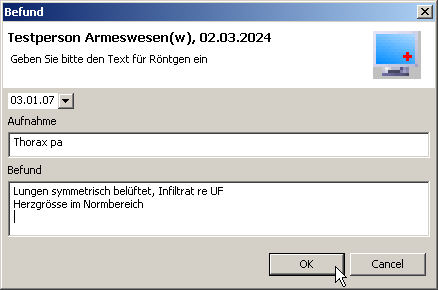
\includegraphics[width=3in]{images/befunde6.png}
% befunde6.png: 438x290 pixel, 96dpi, 11.59x7.67 cm, bb=0 0 328 217
\end{flushleft}
Sie sehen jetzt Ihre bei der Konfiguration angegebenen Messzeilen, ein- oder mehrzeilig. Mit Klick auf OK wird der neue Eintrag übernommen. Mit Doppelklick können Sie ihn wieder öffnen.

Im Fall eines berechneten Wertes können Sie die Rechnung durch Klicken auf den blauen Titel auslösen:\
\begin{center}
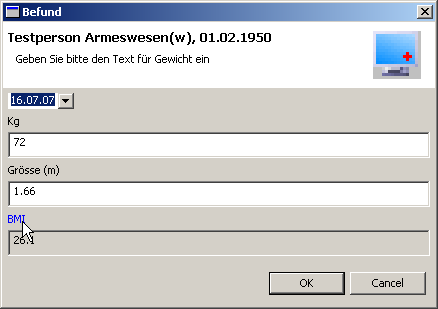
\includegraphics{images/befunde8}
\end{center} 

\subsection{Text-Platzhalter}
\index{Platzhalter} \index{Textfelder}
Befunde können auch in Platzhalter von Textdokumenten eingefügt werden. Sie müssen hierzu die Syntax wie unter 'Daten aus externen Plugins' beschrieben (\ref{datenfelder_extern}, S. \pageref{datenfelder_extern}) anwenden. Der Schlüsselname des Befunde-Plugins ist \textsc{Befunde-Data}.

Um beispielsweise eine Tabelle mit dem Gewichtsverlauf des aktuellen Patienten im aktuellen Dokument einzufügen, setzen Sie folgenden Platzhalter ein:
\begin{verbatim}
    [Befunde-Data:Patient:all:Gewicht]  (um eine Tabelle mit allen Messungen auszugeben)
    [Befunde-Data:Patient:last:Gewicht] (Um nur die letzte Messung auszugeben)
\end{verbatim}
 